%*******************************************************************************
% Macro per il documento corrente
%*******************************************************************************
\newcommand{\sharedPath}{../shared}
\newcommand{\doctitle}{Piano di Progetto}
\newcommand{\docauthor}{\team}

%*******************************************************************************
% Preambolo
%*******************************************************************************
\documentclass[a4paper,10pt,twoside]{book}

%*******************************************************************************
% Codifica e lingua
%*******************************************************************************
\usepackage[utf8x]{inputenc}
\usepackage[T1]{fontenc}
\usepackage[english,italian]{babel}
\usepackage{lmodern}
\usepackage{multirow}
\usepackage{amsmath,eurosym}
%*******************************************************************************
% Qualche macro utile a tutti
%*******************************************************************************
\newcommand{\docRoot}{..}
\newcommand{\inglese}[1]{\foreignlanguage{english}{\textit{#1}}}
\newcommand{\team}{\textsf{EtaBeta\,Software}\xspace}
\newcommand{\caName}{BPM-1.0\xspace}
\newcommand{\customer}{\textsf{Alpha\,\&\,Partners}\xspace}
\newcommand{\mktg}{\inglese{marketing}\xspace}
\newcommand{\bsn}{\inglese{business}\xspace}
\newcommand{\sw}{\inglese{software}\xspace}

%*******************************************************************************
% Figure e immagini
%*******************************************************************************
\usepackage{graphicx}
\graphicspath{{\docRoot/shared/pictures/}}

%*******************************************************************************
% Tabelle
%*******************************************************************************
\usepackage{booktabs}
\usepackage{array}

%*******************************************************************************
% Elenchi puntati personalizzati
%*******************************************************************************
\usepackage{enumitem}

%*******************************************************************************
% Landscape per ruotare le pagine
%*******************************************************************************
\usepackage{pdflscape}

%*************************************************
% Collegamenti intra- e intertestuali
%*************************************************
\usepackage{hyperref}
\hypersetup{%
    colorlinks=false,linktocpage=false,pdfborder={0 0 0},%
    pdfstartpage=1, pdfstartview=FitV,plainpages=false,%
    urlcolor=Black, linkcolor=Black,
    pdfcreator={pdfLaTeX},%
    pdfproducer={pdfLaTeX with hyperref package}%
}

%*************************************************
% Grafica vettoriale
%*************************************************
\usepackage{tikz}
\usetikzlibrary{shadows,arrows,shapes}

%*******************************************************************************
% Altri pacchetti
%*******************************************************************************
\usepackage{xspace} % per spazi condizionali extra
\usepackage{lastpage} % per sapere il numero totale di pagine
\usepackage{microtype} % qualche accorgimento tipografico

% *************************************************
% Intestazioni e piè di pagina personalizzati
% *************************************************
\usepackage{fancyhdr}

% stile normale
\fancypagestyle{normal}{
\fancyhead{}
\fancyhead[RE,LO]{
\sffamily\team
}
\fancyhead[LE,RO]{
\sffamily\leftmark
}
\renewcommand{\headrulewidth}{.4pt}
\cfoot{}
\fancyfoot[LE,RO]{\sffamily
  pag. \thepage{} di \pageref{LastPage}}
\fancyfoot[RE,LO]{\sffamily\doctitle}
\renewcommand{\footrulewidth}{.4pt}
}

% stile per gli indici
\fancypagestyle{toc}{
\fancyhead{}
\renewcommand{\headrulewidth}{0pt}
\cfoot{}
\fancyfoot[RO,LE]{\sffamily\thepage{}}
\fancyfoot[RE,LO]{\sffamily\doctitle{}}
\renewcommand{\footrulewidth}{.4pt}
}

\pagestyle{fancy}
\renewcommand{\sectionmark}[1]{\markboth{#1}{#1}}


%*******************************************************************************
% Inizio documento
%*******************************************************************************
\begin{document}

\pagestyle{empty}
\begin{center}

{\sffamily
Sviluppo e Gestione Progetti\\
a.a. 2012--2013
}

\vskip 1.5cm

{
\setlength{\fboxsep}{.2pt}
\fbox{
\includegraphics[width=\textwidth]{logo}}
}

\vskip .5cm

{\Huge\sffamily\bfseries
\team
}

\vskip 1.5cm

% titolo del progetto
{\Large\sffamily\bfseries
\caName
}

\vskip 1cm

% titolo del documento
\hrule
\vskip 10pt
{\Huge\scshape
\doctitle
}
\vskip 10pt
\hrule

\end{center}

\clearpage
\pagenumbering{roman} 

\tableofcontents{\thispagestyle{toc}}

\clearpage

\pagestyle{normal}
\pagenumbering{arabic}

\chapter{Piano di Progetto}

%\section{Introduzione}

%\subsection{Scopo del documento}

% DESCRIZIONE DI ETA BETA
% \team si configura come una società di consulenza aziendale altamente specializzata in soluzioni basate sul paradigma BPM\@. Il \inglese{focus} della sua attività consiste nell'individuare e integrare le soluzioni di qualità esistenti -- sulla scorta di una profonda conoscenza delle alternative disponibili sul mercato sia nazionale che internazionale e con uno speciale interesse nei confronti delle innovazioni più \inglese{cutting edge} del momento -- integrandole con  soluzioni sviluppate \inglese{ad hoc} per i problemi particolari al fine di adattarsi con una precisione `sartoriale' alle esigenze e alle strategie dei singoli clienti.

% Le soluzioni proposte da \team rendono possibile innovare il proprio modello di \bsn monitorando in tempo reale lo svolgimento dei processi aziendali al fine di adottare misure correttive \inglese{in itinere} e, grazie alla consapevolezza maturata in tale sede, risolvere in maniera permanente le criticità nell'ottica del miglioramento continuo e del BPR (\inglese{Business Process Reengineering}).

% \team nasce nel 2010 con una missione fortemente orientata all'innovazione, allo scopo di fornire soluzioni \sw di alta qualità e a costi `ragionevoli' che mettano i propri clienti nelle condizioni di ottimizzare l'utilizzo delle risorse e migliorare in maniera sostenibile la propria efficienza e la propria competitività in un periodo particolarmente critico per l'economia come quello attuale.

% Il \inglese{team} di \team si compone di due esperti di \bsn \inglese{analysis} e organizzazione aziendale, uno specialista di \inglese{project management} e tre ingegneri del \sw come evidenziato nel diagramma riportato in \figurename~\ref{fig:organigram}.

% L'ambiente di collaborazione multidisciplinare che scaturisce da una simile combinazione di esperti con \inglese{background} afferenti a discipline profondamente differenti ma che nel corso del tempo hanno evidenziato importanti segnali di convergenza permette all'impresa di creare soluzioni apposite da integrare con quelle esistenti per conseguire gli obiettivi primari di pianificare, monitorare e automatizzare la gestione dei processi aziendali migliorandone l'efficienza ma senza sacrificare le spinte all'innovazione e mantenendo un basso profilo di costi.

% \team adotta internamente un \emph{modello integrativo} fortemente orientato al \inglese{commitment} che vede coinvolte al contempo lo sviluppo delle risorse interne, considerate come \inglese{asset} aziendali meritevoli di investimento in formazione continua piuttosto che come mere variabili di costo, e il controllo relativo alla \inglese{compliance} dei dipendenti rispetto agli standard di processo mirando alla costituzione di un ciclo virtuoso in cui le relazioni sociali e la fiducia reciproca sono incoraggiati nel rispetto degli obiettivi e senza perdere di vista il \inglese{focus} sui risultati aziendali.

% Le competenze maturate come analista di organizzazione aziendale e solida esperienza e nella gestione delle risorse umane del titolare consentono di mantenere sotto costante controllo l'operato dei dipendenti al fine di garantire il pieno rispetto della pianificazione e la qualità del risultato finale.






\section{Pianificazione}
\subsection{Work Breakdown Structure}

La Work Breakdown Structure (WBS) costituisce il primo passo verso una buona pianificazione.

La WBS sfrutta il concetto di \textit{``divide et impera''}; essa infatti ha lo scopo di suddividere il lavoro di progetto in parti minori: in questo modo anche i progetti più complessi diventano realizzabili.

La scomposizione avviene in modo gerarchico: il lavoro viene suddiviso in una serie di attività che vengono a loro volta scomposte in sotto-attività di dimensioni più piccole e semplici da gestire, dette Work Package (WP).
La rappresentazione della scomposizione avviene tramite l'uso di un albero, dove i nodi interni rappresentano le attività e le foglie i singoli WP\@.

La WBS permette, tramite la suddivisione del lavoro in segmenti minori, di analizzare tutte le implicazioni del progetto senza tralasciare alcun aspetto. Inoltre, costituisce anche un buon punto di partenza per calcolare costi e benefici del progetto.
La WBS, infine, offre una chiara visione del prodotto finale e del processo complessivo attraverso il quale è stato creato il prodotto.

Si presenta di seguito la definizione della WBS per il progetto\ldots%TODO questo va scritto alla fine, non si può fuffare ora!

Ogni sezione riporta la descrizione dell'attività di primo livello e la descrizione relativa ad ogni suo WP. 

Il \inglese{team} ha scelto di strutturare la WBS seguendo il ciclo di vita del progetto.

\begin{figure}[!h]
  \centering
  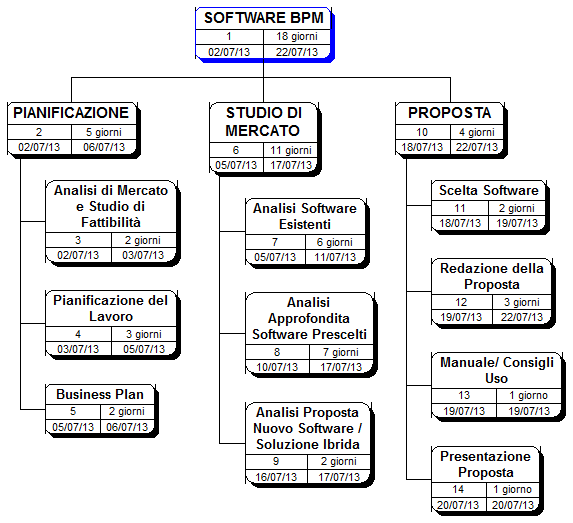
\includegraphics[width=\textwidth]{WBS}
  \caption{Work Breakdown Structure}
\end{figure}

\subsubsection{Pianificazione}
In questa fase devono essere eseguite tutte le attività necessarie alla pianificazione del progetto.
Dovranno pertanto essere individuate ed organizzate tutte le attività da svolgere, i tempi e le risorse necessarie allo sviluppo del progetto. Tale fase comprende anche la stesura del \inglese{Business Plan}.
		
\paragraph{Analisi di mercato e Studio di fattibilità}
\begin{description}
  \item{\bfseries Descrizione:}\\
Questo WP prevede uno studio generale del mercato sui \inglese{software} BPM, con lo scopo di permettere l'organizzazione della pianificazione in base alle informazioni tratte dagli studi.
		
In particolare, lo studio di fattibilità dà al \inglese{team} la possibilità di capire se gli strumenti e le risorse di cui dispone sono sufficienti a garantire il conseguimento dell'obiettivo.

L'analisi, invece, permette di eseguire una corretta pianificazione sulla base di informazioni reali riguardanti il mercato attuale. 
% \item {\bfseries Responsabile:}
  \item{\bfseries Attività:}
  \begin{enumerate}
    \item Ricerche relative ai \sw BPM;
    \item Ricerche sui \inglese{competitor} del mercato;
    \item Ricerche brevettuali.
  \end{enumerate}
  \item  {\bfseries Costo:} \text{\euro} 350,00 
  \item  {\bfseries Tempo di realizzazione:} 2 giorni lavorativi
\end{description}

\paragraph{Pianificazione del lavoro}
\begin{description}
\item{\bfseries Descrizione:}\\
Questa attività prevede la pianificazione del lavoro in seguito allo studio di fattibilità effettuato. Il lavoro deve essere organizzato nelle sue attività e nei suoi tempi.
% \item{\bfseries Responsabile:}
\item{\bfseries Attività:}
	\begin{enumerate}
		\item Stesura WBS;
		\item Stesura OBS;
		\item Matrice delle responsabilità;
		\item Stesura RBS;
		\item Diagramma di Gantt.
  \end{enumerate}
  \item{\bfseries Costo:} \text{\euro} 600,00 
  \item{\bfseries Tempo di realizzazione:} 2 giorni lavorativi
\end{description}

\paragraph{Redazione Business Plan}
\begin{description}
\item{\bfseries Descrizione:}\\
La \team si assume l'incarico di supportare la \customer nella redazione  del Business Plan del piano di sviluppo. Infatti, prevedendo il piano tra i suoi progetti, l'acquisto di \sw BPM, la \customer ha richiesto un intervento dell'azienda alla quale ha commissionato il compito della scelta del \sw.

Pertanto questo WP prevede la collaborazione di \team con la \customer per la redazione del Business Plan. Tale documento è molto importante sia a titolo organizzativo che rappresentativo, del progetto di sviluppo e dell'azienda stessa.
% \item {\bfseries Responsabile:}
  \item  {\bfseries Attività:}
  \begin{enumerate}
		\item Individuazione del contenuto del documento;
		\item Individuazione informazioni necessarie alla stesura del documento;
		\item Analisi del mercato e dei \inglese{competitor};
		\item Studio dell'aspetto finanziario.
	\end{enumerate}
  \item{\bfseries Costo:} \text{\euro} 520,00 
  \item{\bfseries Tempo di realizzazione:} 2 giorni lavorativi
\end{description}

\subsubsection{Studio di mercato}
In questa fase devono essere eseguite tutte le attività inerenti allo studio di mercato sui \sw BPM\@.
Il primo passo da compiere è l'analisi generica del mercato e l'individuazione dei prodotti esistenti. Sarà poi necessario selezionare alcuni \sw atti all'analisi approfondita in modo tale da poter scegliere la migliore soluzione. 

\paragraph{Studio dei \sw esistenti }
\begin{description}
\item{\bfseries Descrizione:}\\
Questo WP prevede l'analisi dei \sw già presenti nel mercato. Si tratta di analizzare le diverse soluzioni già esistenti in commercio ed individuare quelle più adatte all'obiettivo del progetto. 

% \item {\bfseries Responsabile:}
  \item  {\bfseries Attività:}
	\begin{enumerate}
		  \item Analisi generica delle soluzioni \sw già presenti nel mercato;
		  \item Selezione di una lista di \sw da visionare;
		  \item Analisi generale dei \sw.
		\end{enumerate}
  \item  {\bfseries Costo:} \text{\euro} 965,00 
  \item  {\bfseries Tempo di realizzazione:} 6 giorni lavorativi
\end{description}

\paragraph{Studio dei \sw prescelti}
\begin{description}
\item{\bfseries Descrizione:}\\
Questo WP prevede l'analisi dei \sw selezionati. Si tratta di analizzare, studiare e confrontare le prestazioni dei vari \sw sulla base della lista delle funzionalità richieste da \customer.

% \item {\bfseries Responsabile:}
\item  {\bfseries Attività:}
\begin{enumerate}
		\item Individuazione della lista degli aspetti da tenere in considerazione;
		\item Analisi individuale di ogni \sw;
		\item Confronto dei diversi \sw.
		\end{enumerate}

\item  {\bfseries Costo:} \text{\euro} 1.100,00 
\item  {\bfseries Tempo di realizzazione:} 7 giorni lavorativi
\end{description}


\paragraph{Analisi Proposta nuovo \sw o soluzione ibrida }
\begin{description}
\item{\bfseries Descrizione:}\\
Questo WP prevede l'analisi della possibilità della realizzazione di un nuovo \sw o di una soluzione ibrida.

Tale analisi avverrà soltanto dopo aver esaminato i diversi \sw selezionati e la scelta di sviluppare una soluzione \inglese{ad hoc} sarà scaturita dalla possibilità che nessun \sw attualmente in commercio soddisfi pienamente le richieste di \customer.

% \item {\bfseries Responsabile:}
\item  {\bfseries Attività:}
	\begin{enumerate}
    \item Valutazione generale del rispetto dei requisiti posti da \customer;
	  \item Valutazione di costi e benefici della creazione di una soluzione \inglese{ad hoc} \inglese{software}.
	\end{enumerate}
\item  {\bfseries Costo:} \text{\euro} 335,00 
\item  {\bfseries Tempo di realizzazione:} 2 giorni lavorativi
\end{description}

\subsubsection{Proposta}
In questa fase devono essere eseguite tutte le attività inerenti alla stesura delle proposta. Deve essere scelto il prodotto da proporre e individuato il modo per farlo. Si prevede inoltre di realizzare un piccolo manuale per l'uso del prodotto \sw.

\paragraph{Scelta \sw}
\begin{description}
\item{\bfseries Descrizione:}\\
Questo WP rappresenta un punto cruciale. Dalla scelta del \inglese{software} dipende il contenuto della proposta che sarà presentata.

Si tratta quindi di decidere  nel migliore dei modi quel è il \inglese{software} BPM più adatto alle esigenze richieste di \customer.

% \item {\bfseries Responsabile:}
\item  {\bfseries Attività:}
	\begin{enumerate}
		\item Valutazione rispetto ai requisiti obbligatori concordati con \customer;
		\item Valutazione rispetto ai requisiti desiderabili concordati con \customer;
		\item Decisione definitiva con i responsabili.
		\end{enumerate}

\item  {\bfseries Costo:} \text{\euro} 345,00 
\item  {\bfseries Tempo di realizzazione:} 2 giorni lavorativi
\end{description}

\paragraph{Redazione della proposta }
\begin{description}
\item{\bfseries Descrizione:}\\
Una volta che la scelta del \sw è avvenuta, sarà necessario presentarla in modo formale all'azienda richiedente. Si noti che la forma con cui presentiamo il lavoro svolto è fondamentale per avere successo e portare a termine gli obiettivi prefissati.

% \item {\bfseries Responsabile:}
\item  {\bfseries Attività:}
	\begin{enumerate}
	\item Individuazione del contenuto della proposta;
	\item Stesura del documento;
	\item Verifica del documento;
 	\item Approvazione del documento.	
	\end{enumerate}

\item  {\bfseries Costo:} \text{\euro} 420,00 
\item  {\bfseries Tempo di realizzazione:} 2 giorni lavorativi
\end{description}

\paragraph{Redazione manuale/Consigli d'uso}
\begin{description}
\item{\bfseries Descrizione:}\\
Questo WP consiste nella stesura di un breve manuale per l'uso del \inglese{software} con il fine di facilitare gli utenti che ne faranno uso.

% \item {\bfseries Responsabile:}
\item  {\bfseries Attività:}
	\begin{enumerate}
	\item Individuazione del contenuto del manuale
	\item Scelta della forma di presentazione
	\item Verifica 
 	\item Approvazione	
	\end{enumerate}

\item  {\bfseries Costo:} \text{\euro} 60,00 
\item  {\bfseries Tempo di realizzazione:}  1 giorno lavorativo
\end{description}

\paragraph{Presentazione proposta}
\begin{description}
	\item{\bfseries Descrizione:}\\
Questo WP costituisce la conclusione di tutto il lavoro di progetto svolto. Si tratta di 		riassumere in una breve presentazione i contenuti del progetto e in particolari i motivi che hanno portato alla scelta di un determinato \inglese{software} BPM.

% 	\item {\bfseries Responsabile:}
	\item  {\bfseries Attività:}
	\begin{enumerate}
		\item Individuazione del contenuto della presentazione
		\item Creazione della presentazione
	\end{enumerate}
	\item{\bfseries Costo:} \text{\euro} 80,00 
	\item{\bfseries Tempo di realizzazione:}  1 giorno lavorativo
\end{description}

\subsection{Organizational Breakdown Structure}
l'Organizational Breakdown Structure (OBS) rappresenta l'organizzazione del progetto rispetto alle risorse umane impiegate in esso.
L'OBS rappresenta una scomposizione gerarchica delle responsabilità di progetto, generata alla scopo di individuare i responsabili di ogni WP.

L'OBS deve essere creata in seguito alla redazione della WBS. Infatti, solo dopo aver tracciato i WP è possibile assegnare loro un responsabile/esecutore.

La creazione della OBS risulta utile sia sotto l'aspetto gerarchico in quanto permette al \inglese{Project Manger} di individuare i responsabili, sia sotto l'aspetto organizzativo degli esecutori materiali delle attività, in quanto facilita la comunicazione tra essi permettendo di capire a chi chiedere cosa. 

\begin{figure}[h!]
  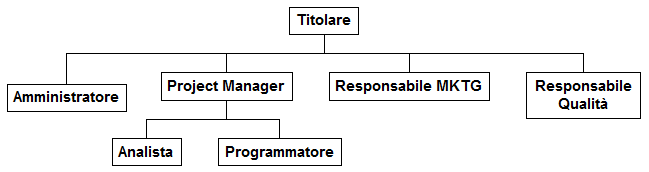
\includegraphics[width=\textwidth]{OBS}
	\caption{Organizational Breakdown Structure}
	\label{fig:obs}
\end{figure}

Come si evince dal diagramma riportato in \figurename~\ref{fig:obs}, tutti i responsabili sono a capo del titolare dell'azienda. Essendo infatti una piccola azienda il controllo, pur essendo distribuito rimane comunque sotto la supervisione del titolare.
Il Project Manager è invece a capo dell'Analista e del Programmatore. 
 
Si precisa inoltre che le risorse umane impiegate nel progetto sono tutte e sole quelle di cui dispone l'azienda \team.

	\subsubsection{Titolare}
	Il Titolare è colui che possiede l'azienda (in tutto o in parte).
	
	\subsubsection{Amministratore}		
	L'amministratore è una figura molto importante dal punto di vista organizzativo. Ogni decisione deve essere approvata da 	tale figura e perciò deve essere messo al corrente di cosa succede sia nelle attività ordinarie che in quelle di progetto.
	
	Egli è responsabile dell'efficienza e dell'operatività dell'ambiente di sviluppo. Controlla inoltre versioni e configurazioni del prodotto.
	
	\subsubsection{Project Manager}
	Il Project Manager ricopre un ruolo determinante nella gestione dei progetti. Questi è infatti responsabile della valutazione, pianificazione, realizzazione e controllo di un progetto.
	
	I suoi compiti più importanti sono:
	\begin{itemize}
		\item Valutazione di costi e benefici del progetto
		\item Pianificazione del progetto
		\item Pianificazione e gestione dei rischi di progetto
		\item Valutazione dello stato di avanzamento del progetto
		\item Adozione di misure correttive qualora l'avanzamento del progetto non corrispondesse alla pianificazione

	\end{itemize}

\subsubsection{Responsabile Marketing}
	Questa figura si occupa della definizione ed applicazione delle strategie di \inglese{marketing}. Il Responsabile Marketing si interessa delle relazioni con i clienti e della promozione delle attività dell'azienda stessa.
	
	Tale figura si occupa inoltre, del monitoraggio dei dati di mercato, degli indicatori e dei canali di vendita, al fine di permettere l'identificazione di nuove opportunità di \bsn. La persona che ricopre il ruolo di Responsabile Marketing deve avere ottime capacità relazionali, manageriali e di \inglese{leadership}. 
	
\subsubsection{Responsabile Qualità}	
	La qualità è fondamentale per avere successo nei progetti. Oggi è una proprietà irrinunciabile, sia per clienti che fornitori. Per i clienti si tratta infatti di un'assicurazione sul prodotto/servizio che acquistano e per i fornitori, invece, costituisce  un punto di distinzione rispetto ai concorrenti.
	
Pur essendo una piccola azienda, \team punta al raggiungimento della qualità, tramite l'adeguamento allo standard ISO/IEC 9001.
Nell'ambito dei progetti aziendali il Responsabile Qualità deve assicurare l'attuazione dei processi volti a garantire il rilascio di un prodotto/servizio che rispetta tutti i requisiti di qualità stabiliti.
	 
\subsubsection{Analista}
	L'Analista ha un ruolo fondamentale nella fase iniziale del progetto. Tale figura deve infatti effettuare lo studio di fattibilità preoccupandosi dell'aspetto tecnico.

Nel caso di specie l'Analista ricopre un ruolo molto importante anche nella fase di sviluppo. Egli sarà, infatti, una delle persone addette alla valutazione dei \inglese{software} esistenti nel mercato e perciò  dalla sua stima dipende in gran parte il successo o il fallimento del progetto.

\subsubsection{Programmatore}
	 Tale ruolo, in generale, dovrebbe limitarsi alla sola attività di codifica seguendo le direttive progettuali per sviluppare il prodotto finale. In questo progetto, essendo l'azienda molto piccola, egli avrà il compito di supportare l'Analista nello studio di fattibilità e di collaborare con quest'ultimo all'analisi dei \sw avvalendosi della propria personale esperienza.

\subsection{Matrice delle responsabilità}
La rappresentazione delle assegnazioni delle responsabilità tramite una matrice permette la definizione del flusso di comunicazioni all'interno della struttura organizzativa del progetto.

La matrice, permette infatti, di individuare all'interno dell'organizzazione non solo i responsabili di una certa attività ma anche quei soggetti che devono essere consultati o informati.

\begin{figure}[!h]
  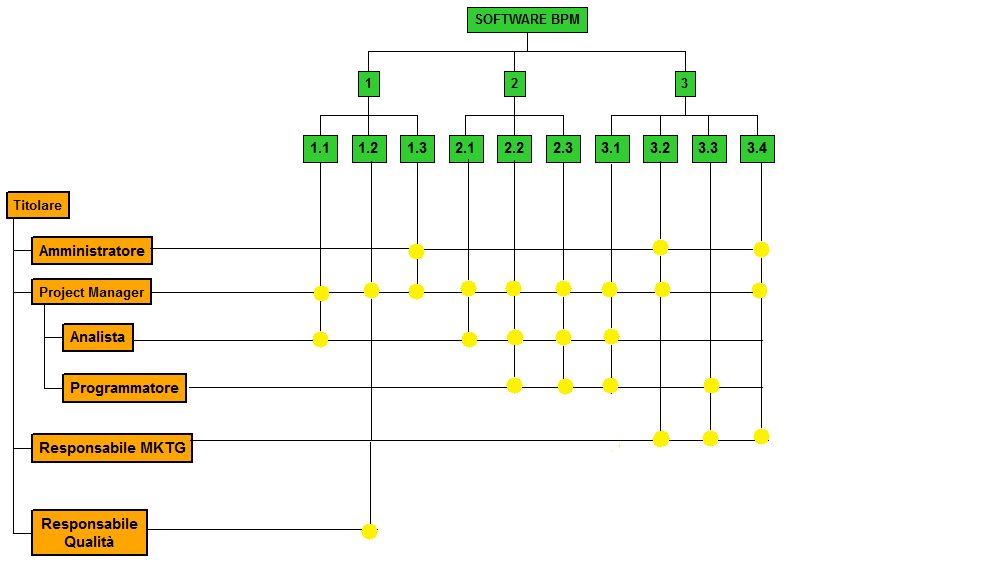
\includegraphics[width=1.25\textwidth]{WBS_OBS}
	\caption{Matrice delle responsabilità e WBS}
	\label{fig:WBS_OBS}
\end{figure} 

\clearpage
\begin{figure}[!h]
  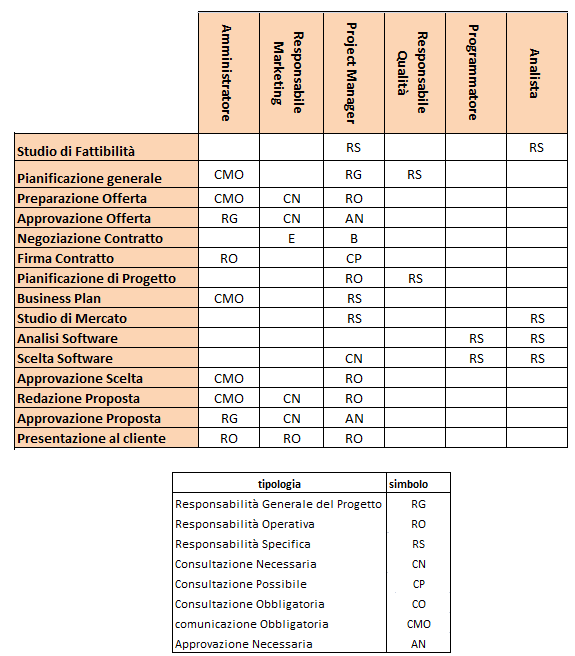
\includegraphics[width=0.9\textwidth]{matrice}
  	\label{fig:MATR}
	\caption{Matrice delle Responsabilità}
\end{figure}

La \figurename~\ref{fig:WBS_OBS} illustra come la matrice delle responsabilità rappresenta l'incrocio tra la WBS e l'OBS. Il diagramma chiarisce infatti chi fa cosa.

La \figurename~\ref{fig:MATR} rappresenta invece la matrice delle responsabilità in modo da individuare anche la specifica responsabilità di ogni figura. Si noti che tale matrice contiene attività molto specifiche, come l'Approvazione, che non si è ritenuto importante inserire nel WBS.

Inoltre si fa notare che per attività di Pianificazione Generale si intende una pianificazione poco precisa che ha il solo fine di capire se l'azienda poteva candidarsi per il capitolato. Infine, per quanto riguarda l'attività di Preparazione Offerta si intende la candidatura stessa del \inglese{team} mentre la Firma del Contratto si riferisce all'approvazione da parte del docente.

\subsection{Resource Breakdown Structure}
Una volta definite quali sono le attività da svolgere e chi ne è responsabile è buona norma effettuare la pianificazione di tutte le risorse necessarie alla svolgimento del progetto, sia umane che strumentali.

Tale organizzazione viene effettuata con lo strumento di pianificazione Resource Breakdown Structure (RBS).
Lo scopo principale di RBS è esplicitare tutte le risorse necessarie e le relazioni che intercorrono tra esse, organizzando queste informazioni in un diagramma gerarchico ad albero e classificandole per categoria.

\begin{landscape}
\vskip 2in

\begin{figure}
\centering
  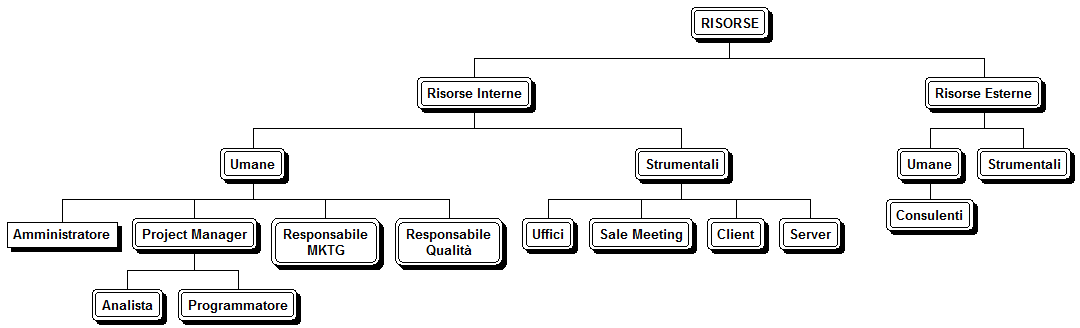
\includegraphics[width=1.5\textwidth]{RBS}
  	
	\caption{Resource Brakedown Structure}
	\label{fig:RBS}
\end{figure}

\end{landscape}

Come si evince dal diagramma riportato in \figurename~\ref{fig:RBS}, le risorse necessarie sono state suddivise gerarchicamente in interne ed esterne, e a loro volta in umane e strumentali. Tale suddivisione permettere di capire dove collocare ogni risorsa necessaria al progetto.

Si noti che vengono considerate esclusivamente le risorse che comportano un costo di cui si dovrà rientrare con gli utili generati dal progetto. Di conseguenza non sono menzionate risorse come \sw con licenza gratuita.

\subsection{Pianificazione Temporale}
Per la pianificazione temporale si utilizza il diagramma di Gantt. Tale diagramma rappresenta infatti l'evoluzione del progetto su scala temporale.

Il Gantt costituisce non solo un ottimo strumento di pianificazione ma anche un buon strumento di controllo che permette in ogni momento di verificare lo stato di avanzamento del progetto rispetto a tempi ed attività pianificate.

Esso è costituito da un asse orizzontale, sul quel viene rappresentato l'arco temporale totale del progetto e un asse verticale, sul quale sono rappresentate tutte le attività ed i singolo WP che costituiscono il progetto.

\begin{figure}[!h]
  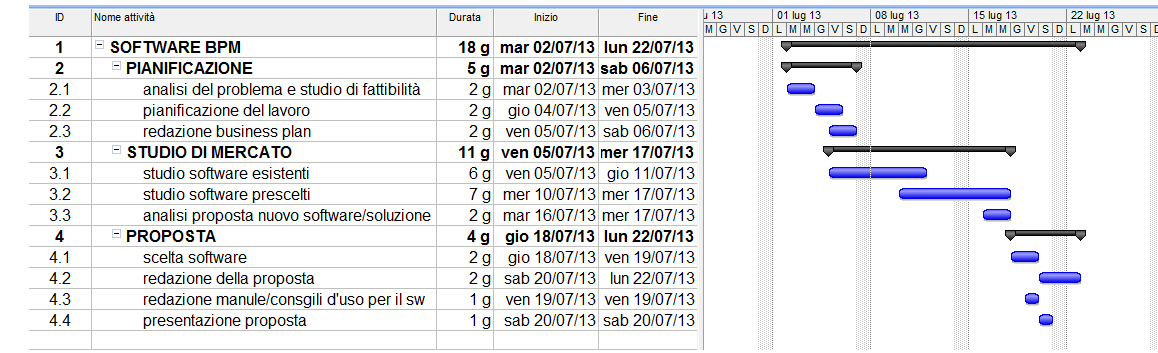
\includegraphics[width=\textwidth]{gantt}	
  	\label{fig:gantt}
	\caption{Diagramma di Gantt}
\end{figure}

\clearpage

\section{Aspetto Economico Finanziario}
Il lato economico costituisce l'aspetto primario di ogni organizzazione che abbia scopo di lucro.

È infatti fondamentale avere un utile sufficientemente remunerativo alla fine del progetto. A tale scopo è finalizzata la stima dei costi relativi al progetto. Tale attività è molto delicata in quanto da essa dipende il reale utile che si ottiene. Infatti, se vi è una sottostima dei costi, l'azienda non avrà utile e nel caso peggiore avrà una perdita. È anche vero, però, che se vi è una sovrastima dei costi, l'azienda non potrà essere competitiva nel mercato.

Il processo di stima avviene calcolando il costo per ogni WP individuato durante il processo di creazione del WBS.

\subsection{Ruoli e Costo }
La seguente tabella espone i costi orari per ogni ruolo individuato.
\begin{table}[!h]
\footnotesize
\centering
\begin{tabular}{|p{.25\textwidth}|c|c|}
\hline
\textbf{Ruolo}& \textbf{Costo Medio} \\
\hline
Amministratore			& \text{\euro} 40,00\\
\hline
Project Manager			& \text{\euro} 30,00\\
\hline
Responsabile MKTG		& \text{\euro} 25,00\\
\hline
Responsabile Qualità	& \text{\euro} 20,00\\
\hline
Analista				& \text{\euro} 25,00\\
\hline
Programmatore			& \text{\euro} 15,00\\
\hline
Consulente				& \text{\euro} 30,00\\
  

\hline
\end{tabular}
\caption{costo Pianificazione}\label{tab:pianificazione}
\end{table}

Si noti che tutte le risorse sono interne ad eccezione del consulente. 

\subsection{Costi per Attività}

\subsubsection{Pianificazione}
Per l'attività di Pianificazione il costo previsto è di \textbf{ \text{\euro}1.470,00 }\\	
I costi per ogni WP della Pianificazione sono riassunti nella seguente tabella.
\begin{table}[!h]
\footnotesize
\centering
\begin{tabular}{|p{.25\textwidth}|c|c|c|c|c|c|c|}
\hline
\textbf{Attività}& \textbf{AM} & \textbf{RMKTG} & \textbf{PM} & \textbf{RQ} & \textbf{PRG} & \textbf{AN} & \textbf{Costo}  \\
\hline
analisi del problema e studio di fattibilità  & & & 5& & & 8& \text{\euro} 350,00\\
pianificazione del lavoro	 				  & & &	16&	6& & & \text{\euro} 600,00 \\	
redazione Business Plan						& 1 & &16& & & &  	\text{\euro} 520,00 \\			  
\hline
\scshape{}pianificazione   							& 1 & &37 &	6 &	&	8 &	\textcolor{red}{ \text{\euro}1.470,00 }\\		 
\hline
\end{tabular}
\caption{costo Pianificazione}\label{tab:pianificazione}
\end{table}

\begin{table}[!h]
\footnotesize
\centering
\begin{tabular}{|p{.25\textwidth}|c|c|c|c|c|c|c|}
\hline
\textbf{Attività}& \textbf{AM} & \textbf{RMKTG} & \textbf{PM} & \textbf{RQ} & \textbf{PRG} & \textbf{AN} & \textbf{Costo}  \\
\hline
analisi del problema e studio di fattibilità  & & & 5& & & 8& \text{\euro} 350,00\\
pianificazione del lavoro	 				  & & &	16&	6& & & \text{\euro} 600,00 \\	
redazione Business Plan						& 1 & &16& & & &  	\text{\euro} 520,00 \\			  
\hline
\scshape{}pianificazione   							& 1 & &37 &	6 &	&	8 &	\textcolor{red}{ \text{\euro}1.470,00 }\\		 
\hline
\end{tabular}
\caption{costo Pianificazione}\label{tab:pianificazione}
\end{table}

\subsubsection{Studio di Mercato}

Per l'attività di Studio di Mercato il costo previsto è di \textbf{ \text{\euro}2.300,00 }\\	
I costi per ogni WP della Studio di Mercato sono riassunti nella seguente tabella.

\begin{table}[!h]
\footnotesize
\centering
\begin{tabular}{|p{.25\textwidth}|c|c|c|c|c|c|c|}
\hline
\textbf{Attività}& \textbf{AM} & \textbf{RMKTG} & \textbf{PM} & \textbf{RQ} & \textbf{PRG} & \textbf{AN} & \textbf{Costo}  \\ 
            
\hline
studio software esistenti & & & 1& & 24& 23& \text{\euro} 965,00\\
studio software prescelti	 				  & & &	&	&40 &16 & \text{\euro} 1.000,00 \\	
analisi proposta nuovo SW/soluzione ibrida 					  & & &2 & 	&5	&  8  &  	\text{\euro} 335,00 \\			  
\hline
\scshape{}studio di mercato  							& 1 &  &3 & &69	&47	&	\textcolor{red}{ \text{\euro}2.300,00 }\\		 
\hline
\end{tabular}
\caption{costo Studio di Mercato}\label{tab:mercato}
\end{table}

\subsubsection{Proposta}
Per l'attività di Redazione della Proposta il costo previsto è di \textbf	{ \text{\euro} 905,00 }	
I costi per ogni WP della Redazione della Proposta sono riassunti nella seguente tabella.

\begin{table}[!h]
\footnotesize
\centering
\begin{tabular}{|p{.25\textwidth}|c|c|c|c|c|c|c|}
\hline
\textbf{Attività}& \textbf{AM} & \textbf{RMKTG} & \textbf{PM} & \textbf{RQ} & \textbf{PRG} & \textbf{AN} & \textbf{Costo}  \\ 
\hline
scelta software			& & & 3&	& 7&	6& 	\text{\euro} 345,00 \\
redazione proposta & 1&	8&	6& & & & 	 \text{\euro} 420,00 \\
redazione manuale / consigli d'uso & & & & & 					4 && 	\text{\euro} 60,00 \\	
presentazione proposta		 & & 2&  	1	& & 	& & 		 \text{\euro} 80,00 \\	
\hline
\scshape{}proposta  							& 1  &10 &10& &	4&	6&	\textcolor{red}{ \text{\euro} 905,00 }\\		 
\hline
\end{tabular}
\caption{costo Redazione Proposta}\label{tab:proposta}
\end{table}	
	
	
\subsubsection*{Consulenza}

Si noti che nelle tabelle relative alle attività non sono inclusi i costi inerenti alla figura del consulente. Il \inglese{team} ha infatti deciso di trattarli a parte. La seguente tabella indica i costi che \team prevede di sostenere per le spese di consulenza in ogni fase.
	
\begin{table}[!h]
\centering
\begin{tabular}{|l|c|c|}
\hline
\textbf{Attività}& \textbf{Consulente} & \textbf{Costo}  \\           
\hline
\scshape{}pianificazione		& 1& \text{\euro} 30,00 \\
\scshape{}studio di mercato 	& 5& \text{\euro} 150,00 \\
\scshape{}proposta 			& &	\text{\euro} 60,00 \\	
\hline
Totale				& 6& \text{\euro} 180,00 \\	
\hline
\end{tabular}
\caption{costo Consulenza}\label{tab:consulenza}
\end{table}

Come si evince dalla tabella~\ref{tab:consulenza} il costo stimato per le spese di consulenza ammonta a \textbf{\text{\euro} 180,00}.

\subsection{Costo Totale}

Il costo totale stimato ammonta quindi a \textbf	{ \text{\euro} 4.855,00 }.
Sarà perciò necessario richiedere un corrispettivo maggiorato di una cifra che possa essere sufficientemente remunerativa ma che allo stesso tempo permetta a \team di essere competitiva nel mercato.


\section{Gestione dei Rischi}
Un rischio è un evento incerto o una condizione di incertezza che se accade determina un effetto positivo o negativo sull'obiettivo di progetto.
La gestione dei rischi è fondamentale in un progetto. Infatti, da una gestione corretta o errata del rischio dipende il successo o il fallimento del progetto.
È quindi necessario individuare quali rischi possono verificarsi durante il progetto e pianificare tecniche e strategie per evitare o, nel caso peggiore, mitigare tali rischi.

La valutazione dei rischi non deve essere un processo statico ma dinamico. Non è infatti sufficiente individuare rischi e tattiche all'inizio del progetto ma è necessario effettuare azioni di controllo costanti. 

\subsection{Analisi dei rischi}

\newcommand{\hi}{\textsc{alta}}
\newcommand{\lo}{\textsc{bassa}}
\newcommand{\med}{\textsc{media}}
Per rendere efficace l'analisi di ogni rischio si è deciso di quantificarlo mediante un apposita scala di valutazione sia dal punto di vista della probabilità che il rischio si manifesti (livello), sia il suo grado di incidenza sul progetto stesso (impatto).

\begin{table}[h!]
\centering
\begin{tabular}{|l|c|}
\hline
Probabilità& Descrizione\\
\hline
\hi & probabilità elevata che si verifichi\\
\med & probabilità equivalente nel verificarsi o meno\\
\lo & probabilità bassa che si verifichi\\
\hline
\end{tabular}
\caption{Probabilità e Descrizione probabilità di un rischio}\label{tab:livellorischi}
\end{table}
\begin{table}[h!]
\centering
\begin{tabular}{|c|c|}
\hline
Scala& Descrizione  \\
\hline
5 & conseguenze molto gravi\\
4 & conseguenze gravi\\
3 & conseguenze medio-gravi\\
2 & conseguenze minimali\\
1 & nessuna/lievi conseguenze\\
\hline
\end{tabular}
\caption{Scala e descrizione delle conseguenze di un rischio}\label{tab:impattorischi}
\end{table}

\subsection{Rischi relativi al Personale}
\begin{description}
	\item{\scshape\bfseries Analisi:}\\
	Durante la realizzazione del progetto è probabile che alcuni membri del team siano soggetti a problemi fisiologici e/o sovvengano impegni personali improrogabili che porterebbero ad una sicura modifica della pianificazione del lavoro collettivo.
	
	L'impatto di tale rischio è variabile in base al soggetto mancante, in quanto può essere assegnato ad un'attività più o meno importante all'interno del progetto. 
	\item{\scshape\bfseries Probabilità:} \med
	\item{\scshape\bfseries Impatto:} variabile
	\item{\scshape\bfseries Strategia di Gestione:}\\
	Per mitigare gli effetti di tali fenomeni è ragionevole prima di tutto pianificare i tempi di lavoro personali in modo da lasciare un lasco temporale tra un attività e l'altra.
	
Purtroppo, data la scarsità di tempo a disposizione, si dispone in questo caso di poco tempo margine. Tuttavia, essendo il periodo che impegnerà il \inglese{team} breve, vi è una cospicua probabilità che le attività procedano come pianificate.
	
Ovviamente anche adottando tali accorgimenti si potrà generare la situazione in cui un componente risulti impossibilitato a svolgere il proprio compito, in tal caso è buona norma che tutti i membri siano ben preparati (conoscenza del dominio e delle metodologie di lavoro) nel caso sia necessaria la sostituzione momentanea del soggetto.
\end{description}

\subsection{Rischi relativi alla tecnologia}
\begin{description}
	\item{\scshape\bfseries Analisi:}\\
	Per ovvie ragioni di inesperienza da parte di tutto il team buona parte delle competenze tecnologiche richieste per la realizzazione del progetto risultano sconosciute.
	\item{\scshape\bfseries Probabilità:} \hi 
	\item{\scshape\bfseries Impatto:} 3 
	\item{\scshape\bfseries Strategia di Gestione:}\\
	Le lacune saranno colmate tramite la personale consultazione di materiale presente in rete. Inoltre, ogni persona provvederà ad aggiornare costantemente gli altri membri del \inglese{team} sul lavoro svolto.
\end{description}

\subsection{Rischi relativi all'errata stima di risorse}
\begin{description}
	\item{\scshape\bfseries Analisi:}\\
	L'errata pianificazione del lavoro fa parte dell'ovvia inesperienza del team, e in particolare di chi ricopre il ruolo di Project Manager. Tali errori possono portare ad uno sbilanciamento dei costi (sia in eccesso che in difetto) che andrà ad incidere sul bilancio finale.
	\item{\scshape\bfseries Probabilità:} \med
	\item{\scshape\bfseries Impatto:} 3 
	\item{\scshape\bfseries Strategia di Gestione:}\\
	Per mitigare gli effetti di tali rischi il \inglese{team} ha cercato di fare ricerche molto approfondite sugli argomenti e ha effettuato una pianificazione leggermente ``pessimistica''. In questo modo viene ridotta la probabilità di incorrere ad eventuali perdite che minerebbero la solidità economico-finanziaria dell'azienda.
\end{description}

\subsection{Rischi relativi al mercato}
\begin{description}
	\item{\scshape\bfseries Analisi:}\\
	Il \inglese{team} non ha nessuna esperienza sulla situazione di mercato dei \inglese{software} BPM\@. Tale carenza, purtroppo, può incidere molto sulla tempistica di realizzazione del progetto.
	\item{\scshape\bfseries Probabilità:} \hi
	\item{\scshape\bfseries Impatto:} 3 
	\item{\scshape\bfseries Strategia di Gestione:}\\
	Per mitigare gli effetti di tali rischi il \inglese{team} potrà avvalersi di eventuali consulenti e dell'aiuto del docente.
\end{description}	

%*******************************************************************************
% STUDIO DI MERCATO
%*******************************************************************************

\chapter{Studio di Mercato}
\section{Introduzione}
\subsection{Cosa sono i software BPM}
	
Tutte le aziende lavorano per processi: essi sono il cuore e l'anima di ogni organizzazione.
		
Uno dei punti che determinano il successo di un'azienda è costituito dall'organizzazione e gestione dei processi stessi. I \sw BPM permettono di gestire i processi facendo uso della tecnologia. 
		
Si tratta di \sw all'avanguardia che permettono la pianificazione, la gestione ed il monitoraggio dei processi.
I \sw BPM permettono  ai \inglese{leader} di grandi e piccole aziende, di avere una migliore comprensione, di prendere decisioni più rapide e cosa più importante, di eliminare il caos e l'inefficienza che possono avere un'incidenza sul vantaggio competitivo di un'azienda.

Spesso questi \sw permettono di interagire con altri \sw gestionali, database o PIM\@.\footnote{I \inglese{Personal Information Manager} sono \sw che permettono di organizzare un certo tipo di informazioni personali per migliorare la produttività aziendale. In genere questi \sw sono usati per gestire \inglese{email} e rubriche.}

Infine, i \sw BPM permettono una corretta gestione dei flussi informativi. Infatti, almeno il 70\% delle informazioni non sono sufficientemente strutturate e quindi perdono valore, come emerge da alcuni studi come ad esempio \cite{mazzolari:bpmita}. Grazie ai \sw BPM è possibile massimizzare l'apporto di valore fornito dalle informazioni ed essere quindi competitivi nel mercato.

\subsection{Vantaggi}
L'adozione di una soluzione di BPM ha il vantaggio di comportare un incremento dell'efficienza a seguito dell'automazione dei processi nonché l'eliminazione degli \inglese{step} intermedi non necessari dovuta all'acquisizione di maggior consapevolezza derivante dalla formalizzazione dei processi aziendali in modelli astratti (situazione corrente `as is').

Implicando la standardizzazione del metodo di lavoro, l'implementazione di un \inglese{workflow management system} conseguenza implicita dell'adozione di un BPM permette di utilizzare di strumenti di verifica e di generazione automatica di \inglese{report} sulle attività ordinarie dell'azienda che consentono di monitorare gli indicatori chiave con estrema accuratezza. Si tratta di condizioni imprescindibili per una buona pianificazione e per l'ottimizzazione dei processi (situazione ideale o `to be') e per passare dalla semplice modellazione dei processi aziendali (\bsn \inglese{process modeling}) a una rivisitazione critica degli stessi (\bsn \inglese{process reengineering}).

In altre parole, i \sw BPM permettendo un'attenta organizzazione ed un continuo controllo dei processi, consentono di ottimizzare la produttività dell'azienda e di ottenere un alto livello di qualità. Inoltre, disponendo delle funzionalità di automatizzazione di alcuni processi, si acquisisce velocità e si rende così l'azienda molto più competitiva nel mercato.

La gestione della non-linearità dei processi, inoltre, denota la flessibilità di tali sistemi, che sono in grado di soddisfare le istanze di modellazione di situazioni che non sono prevedibili aprioristicamente, per adattarsi ai cicli di vita di sempre più ridotte dimensioni per la gestione degli ordini e a un ambiente competitivo in costante evoluzione.

Infine, tramite una gestione controllata dei processi, è possibile incrementare l'efficienza anche in caso di \inglese{workflow} collaborativi, rendendo più trasparente lo scambio di informazioni fra la totalità dei soggetti coinvolti, la condivisione della conoscenza nonché la drastica riduzione dei tempi di accesso alle basi di conoscenza aziendali, incrementandone al contempo l'utilità e le dimensioni perché il flusso di lavoro diviene tracciato, codificato e ripetibile anche in caso di situazioni potenzialmente complesse in maniera indipendente dalla soggettività e dall'esperienza degli incaricati.

Possiamo quindi riassumere i vantaggi che scaturiscono dall'adozione di \sw BPM nel seguente elenco:

\begin{itemize}
	\item miglioramento dell'efficienza dei processi
	\item miglioramento del flusso informativo
	\item controllo coordinato e continuativo dello stato dei processi
	\item miglioramento nella pianificazione del lavoro
	\item attivazione più veloce di interventi correttivi
	\item maggior flessibilità verso situazioni non prevedibili
	\item dematerializzazione dei documenti 	
\end{itemize}
	
\subsection{Cosa offre il mercato}\label{sec:currentmarket}
Attualmente il mercato offre diverse soluzioni, sia gratuite che a pagamento, più, o meno, complete.	
Dall'analisi di mercato effettuata, emerge che in generale, le piccole aziende si affidano alle soluzioni gratuite, alcune delle quali sembrano coprire la maggior parte dei requisti richiesti da tali aziende. Le organizzazioni più complesse, invece, preferiscono acquisire \sw non gratuiti perché a volte risultano essere più completi ed adatti ad organizzazioni più grandi.

Occorre tuttavia tenere presente che nel mercato vi sono \sw distribuiti con una licenza \inglese{open source} e gratuiti, come \swname{Bonita BPM}, che sono in grado di gestire situazioni molto complesse e offrono numerose funzionalità anche di alto livello come parte del pacchetto di base per cui non è necessario sostenere alcun costo di acquisizione.
 
I \inglese{leader} attuali del mercato mondiale, in particolare quello legato alle soluzioni \sw a pagamento, sono grandi colossi del calibro di \swname{IBM}, \swname{Microsoft} e \swname{Oracle}. Tali organizzazioni hanno compreso fin da subito la necessità di offrire alle aziende \sw per la gestione di processi e si sono affermate nel tempo offrendo soluzioni con funzionalità ad alto livello che permettono anche l'interazione con \sw di terze parti.\footnote{%
Un esempio dell'interoperabilità tra le soluzioni offerte e applicazioni esterne è rappresentato da \swname{Bonita Open Solution} che permette, sottoscrivendo un abbonamento di tipo `\textsf{efficiency}', l'interfacciamento con applicativi \swname{SAP}.
}

Il seguente elenco riporta i \inglese{leader} del settore in ordine di rilevanza:
\begin{enumerate}
  \item \swname{IBM}
  \item \swname{Oracle}
  \item \swname{Microsoft}
\end{enumerate}

\swname{IBM} si configura come \inglese{leader} mondiale in vari segmenti, tra cui \inglese{Database Management}, \inglese{Enterprise Content Management} (ECM), \inglese{Customer Data Integration}, \inglese{Information Integration}, \inglese{Information On Demand} e, in generale, Service Oriented Architecture (SOA), operando in 173 paesi ed è presente in Italia dal 1927 svolgendo anche attività di sviluppo software, che fanno capo al \inglese{Rome Tivoli Laboratory}.

Nel campo della \bsn \inglese{intelligence} sono state particolarmente significative le acquisizioni di \swname{Lotus} nel 1995, \swname{Lombardi} nel 2005, \swname{MRO} (marchio \swname{Tivoli}) e \swname{FileNet} nel 2006 nonché \swname{Cognos} nel 2008. Il \inglese{portfolio} soluzioni della divisione \swname{IBM Software Group} comprende allo stato attuale \inglese{brand} fra i quali si menzionano \swname{Information Management}, \swname{Lotus}, \swname{Rational}, \swname{Tivoli}, \swname{WebSphere} e \swname{Product Lifecycle Management}.

\swname{Microsoft} si colloca nel mercato con una soluzione di gestione di database (\swname{Microsoft SQL Server}), collaboraborazione e condivisione di contenuti aziendali (\swname{Microsoft SharePoint}) e la \inglese{suite} di produttività individuale \swname{Microsoft Office}.

\swname{Oracle} si colloca nel mercato applicazioni di \bsn \inglese{intelligence} con prodotti propri e ha rafforzato ulteriormente la propria posizione di dominanza con l'acquisizione di \swname{Hyperion} che risale al 2007. Il risultato è una combinazione completa di strumenti di pianificazione, modellazione delle opzioni strategiche, allineamento organizzativo e reportistica strettamente integrati e funzionali. Attualmente, oltre 12.000 aziende in 91 paesi si affidano a soluzioni \swname{Oracle} per migliorare la comprensione del proprio \bsn e per la realizzazione di iniziative di \inglese{Enterprise Performance Management} (EPM).

Fra le altre società presenti sul mercato, vale la pena di menzionare \swname{SAP}, \swname{Fujistu} e \swname{HP}.

\swname{SAP} è presente con soluzioni di \inglese{data warehousing} come \swname{SAP HANA} e \swname{Sybase IQ} e \sw di monitoraggio e notifica dei processi aziendali (\swname{SAP BusinessObjects Event Insight}) attraverso il controllo degli indicatori di processo  e accordi sul livello di servizio (di tipo prestazionale).

\swname{Fujitsu}, dal canto suo, fornisce soluzioni per la gestione di grandi moli di dati aziendali attraverso la \inglese{suite} \swname{EternusSF} e per l'organizzzione e l'allineamento di risorse informatiche e \inglese{cloud-based} con i prodotti della linea \swname{ServerView}.

\swname{HP} partecipa con prodotti come \swname{HP Business Decision Applicance} e \swname{HP Data Warehouse Appliance} orientati principalmente alle gestione delle informazioni aziendali e all'\inglese{data mining} al fine di facilitare le attività di \inglese{decision making}, integrandosi strettamente con i prodotti \swname{Microsoft} più diffusi per la memorizzazione delle informazioni, come \swname{Microsoft SQL Server}.

Dagli studi di mercato emerge che le maggiori problematiche in questo settore riguardano la difficoltà delle piccole piccole/medie imprese a stare al passo con un mercato sempre più dinamico e la necessità di applicare la cosiddetta `modalità a latenza zero'.\footnote{Con tale espressione si intende l'accesso e la visibilità dello stato di avanzamento dei processi in tempo reale.}

Inoltre si stanno attualmente aprendo della opportunità anche per il settore della Pubblica Amministrazione che si pone l'obiettivo di offrire servizi di qualità.

Infine, molti dei \sw attualmente presenti nel mercato integrano un sistema di gestione documentale in conformità al formato sostitutivo previsto per legge.

Come si evince dal grafico riportato in \figurename~\ref{fig:tipologie}, la quota maggioritaria delle aziende che fanno utilizzo di \sw BPM è detenuta dalle società di consulenza come \customer che ha richiesto a \team di valutare una soluzione che la supporti nello svolgimento delle proprie attività. A seguire, si collocano le \sw \inglese{house} con una quota del 25\%, mentre la categoria dei \inglese{System Integrator} si attesta al 10\%.

\begin{figure}[H]
  \centering
  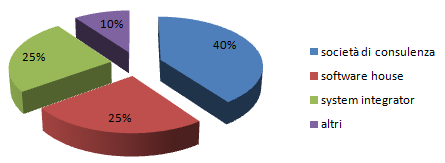
\includegraphics[width=.85\textwidth]{tipologie}
  \caption{Tipologie di aziende che investono in \sw BPM.}
  \label{fig:tipologie}
\end{figure}

\subsection{Prospettiva temporale}
Nel corso dell'ultimo decennio lo scenario del mercato dei \sw ha mostrato una sostanziale evoluzione. Se agli inizi degli anni 2000 si evidenziava una cospicua frammentazione dei fornitori, nel tempo hanno affermato il loro predominio i grandi produttori come \swname{IBM},\swname{Microsoft} e \swname{Oracle}.

Alcune aziende, come la \swname{FileNet}, che prima detenevano una rilevante porzione di mercato sono state assorbite da altre o, come nel caso \swname{Staffware} hanno perso il loro ruolo primario cedendo il passo a \inglese{competitor} di maggiori dimensioni. Sono invece emersi nuovi protagonisti come, ad esempio, \swname{Microsoft} e \swname{Oracle} che all'inizio del decennio detenevano una quota di mercato trascurabile.

\begin{figure}[H]
  \centering
  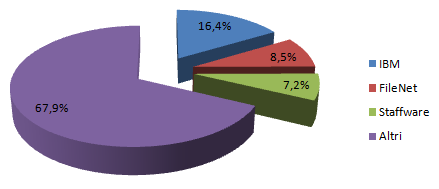
\includegraphics[width=.85\textwidth]{mercato_2000}
  \caption{Situazione del mercato fornitori nel 2000.}
  \label{fig:mercato2000}
\end{figure}

\begin{figure}[H]
  \centering
  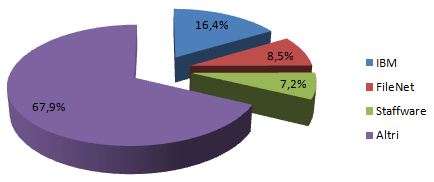
\includegraphics[width=.85\textwidth]{mercato_2012}
  \caption{Situazione del mercato fornitori nel 2012.}
  \label{fig:mercato2012}
\end{figure}

Per quanto riguarda il volume degli investimenti da parte delle aziende nell'acquisizione di \sw BPM è possibile evidenziare un andamento fortemente positivo con la tendenza a mantenere un elevato ritmo di crescita per il futuro.

Il grafico riportato in \figurename~\ref{fig:trend} rappresenta l'andamento mondiale degli investimenti nel settore dell'innovazione tecnologica ed in particolare nei \sw BPM.

\begin{figure}[H]
  \centering
  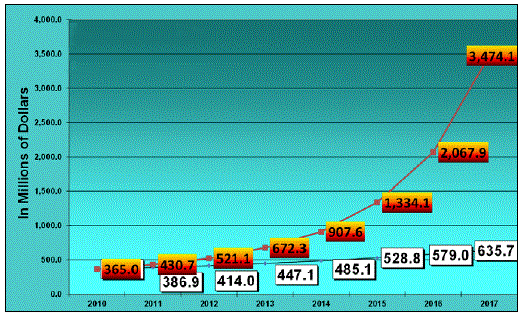
\includegraphics[width=.85\textwidth]{markettrend}
  \caption{Situazione del mercato fornitori nel 2012.}
  \label{fig:trend}
\end{figure}

\subsection{Analisi geotopografica del mercato}% analisi fuffosa
Adottando un approccio territoriale alla segmentazione del mercato, la situazione che emerge rivela una diversificazione del comportamento della domanda fra l'area geografica delle Americhe, l'Europa considerata congiuntamente al Medio Oriente e all'Africa (EMEA) e l'Asia \cite{bea:bpm}. In particolare, considerando il volume degli investimenti, questo risulta decisamente più elevato nella regione americana, dove un investimento dell'entità di 289 milioni di dollari annui denota il carattere prioritario riconosciuto alle soluzioni BPM\@.

La regione europea si colloca al secondo posto con un valore di 137 milioni di dollari, seguita dall'Asia con una spesa pari a 70 milioni di dollari, come illustrato dalla \figurename~\ref{fig:map1}.

\begin{figure}[H]
  \centering
  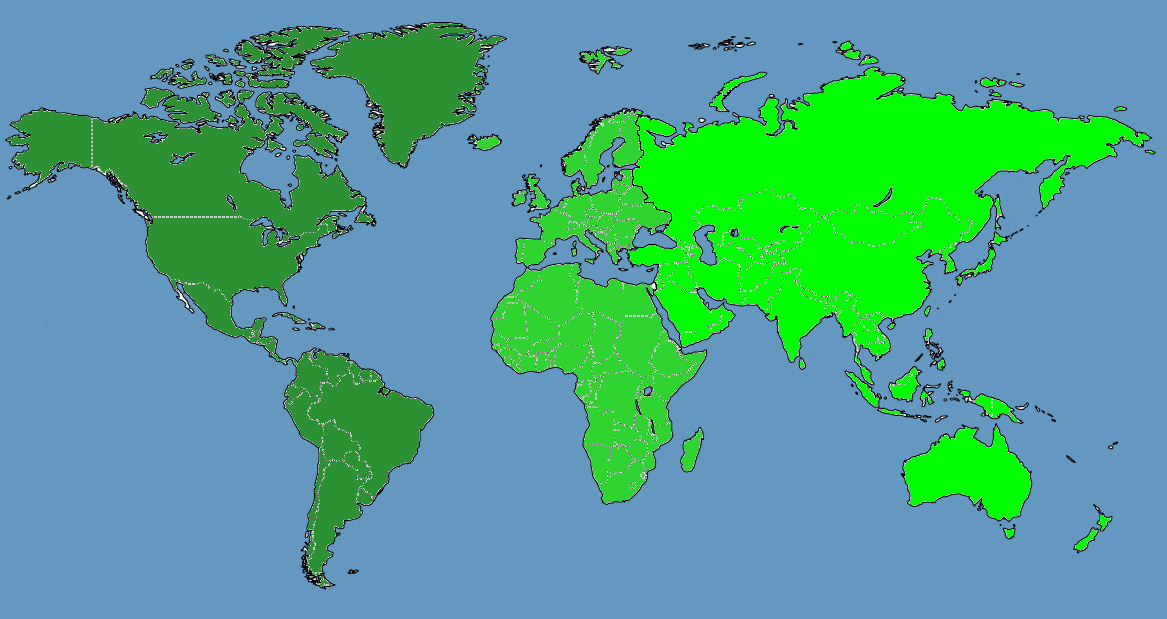
\includegraphics[width=.85\textwidth]{worldmap}
  \caption{Entità degli investimenti in soluzioni BPM nelle diverse aree.}
  \label{fig:map1}
\end{figure}

La situazione delle quote di mercato relativa ai fornitori mostra un sostanziale allineamento con i dati esposti in precedenza, dal momento che la quota maggiore risulta essere detenuta ancora una volta dalle Americhe (58,3\%), mentre Europa e Africa si arrestano ad un livello del 27,6\% e nella regione asiatica il dato rilevato corrisponde al 14,1\%. Tale dato può essere giustificato dal fatto che il mercato attira la specializzazione dei fornitori in questo settore dato il crescente investimento nelle stesse zone.

\begin{figure}[H]
  \centering
  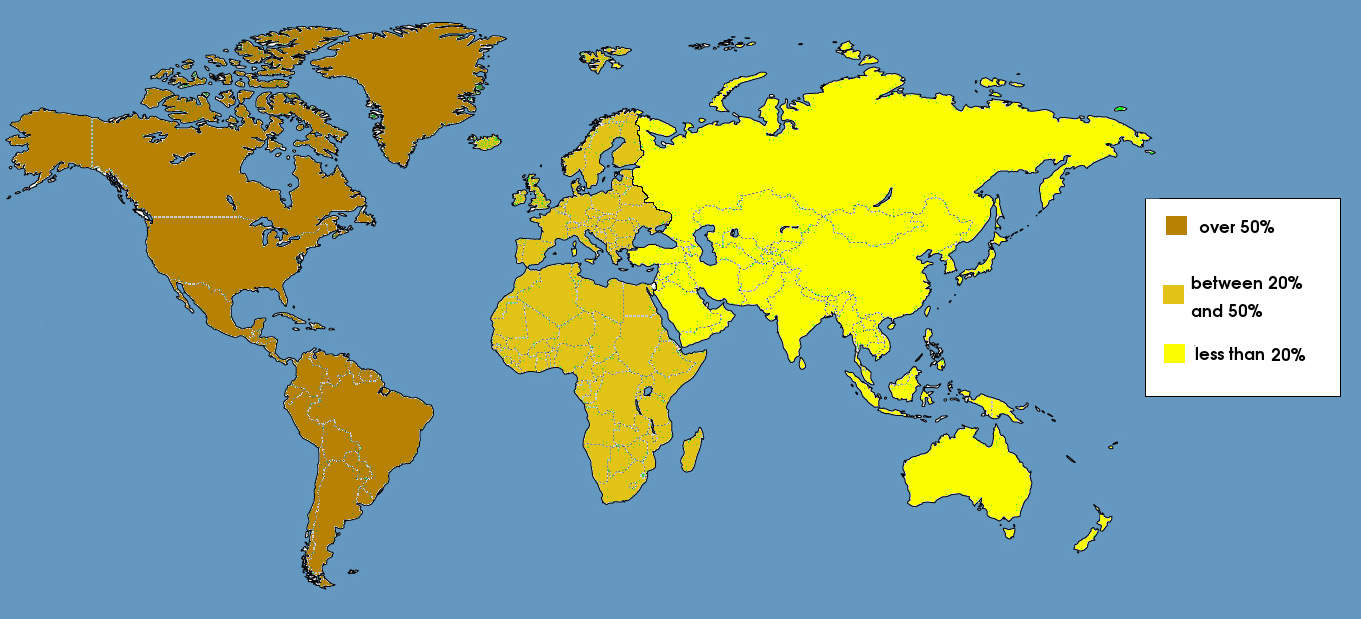
\includegraphics[width=.85\textwidth]{worldmap2}
  \caption{Ripartizione delle quote di mercato nelle vendite di sistemi BPM.}
  \label{fig:map3}
\end{figure}

Un dato più interessante emerge tuttavia incrociando l'analisi sul piano geografico con la prospettiva temporale, considerando la distribuzione sul territorio del tasso di crescita annuale degli investimenti in soluzioni BPM\@. In questo caso, infatti, la regione che comprende Europa, Medio Oriente e Africa mostra un incremento più marcato pari al 45,4\% al di sopra delle Americhe che invece si collocano al 44,8\%. Tale situazione è dovuta al fatto che il settore ha raggiunto un buon livello di maturità nelle Americhe mentre in Europa si tratta di un mercato ancora giovane. Per quanto riguarda, invece, l'estremo oriente, l'Asia e l'Oceania il tasso di crescita denota un incremento annuale nel quinquennio 2006-2011 del solo 37\%.

\begin{figure}[H]
  \centering
  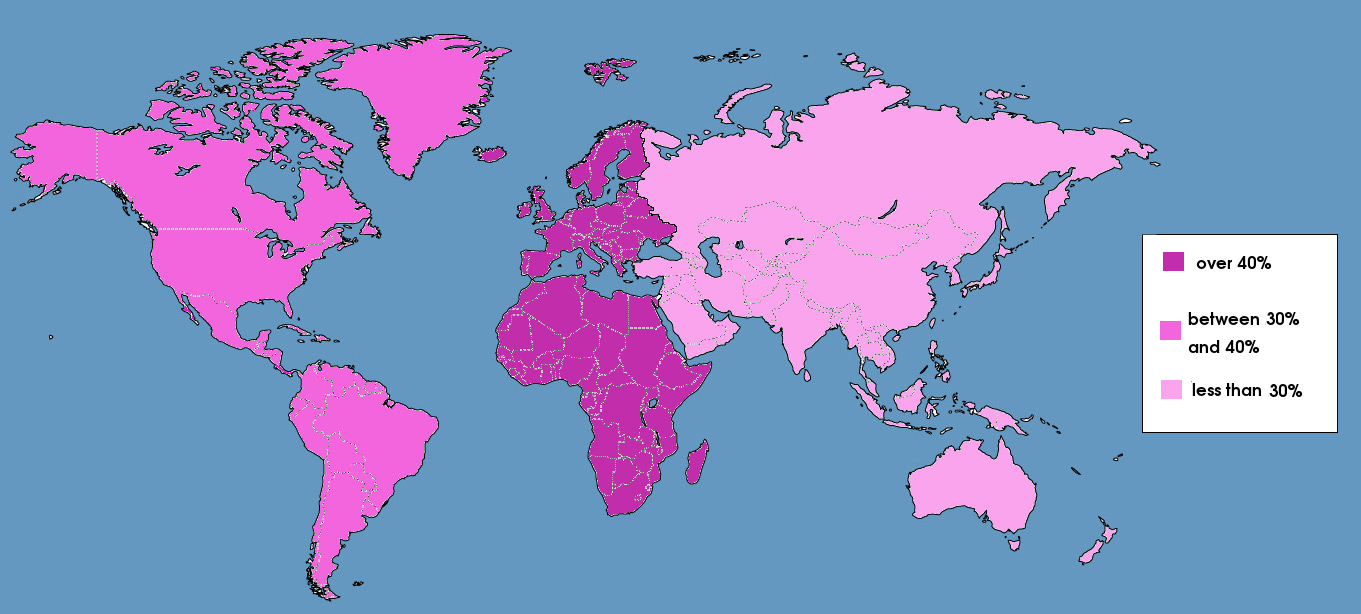
\includegraphics[width=.85\textwidth]{worldmap3}
  \caption{Tasso di crescita annuo nel quinquennio 2006-2011 nel settore BPM.}
  \label{fig:map2}
\end{figure}

\section{Software selezionati}
\subsection{Bonita BPM}
\newcommand{\progname}{\swname{Bonita\,BPM}}
\begin{picture}(0,0)
  \put(250, 10){
\includegraphics[width=.3\textwidth]{bonitasoft_logo}}
\end{picture}

\subsubsection{Descrizione}
Il \sw è distribuito secondo un modello `open core', vale a dire le funzionalità di base sono rilasciate con una licenza \inglese{open source} e possono essere utilizzate e distribuite liberamente, mentre per avere accesso a funzionalità aggiuntive è necessario utilizzare estensioni proprietarie per cui è necessario acquisire una licenza d'uso dal produttore \swname{Bonita BPM}.

Il nucleo `open' dell'applicativo è costituito a sua volta in una serie di moduli grafici e da un motore di esecuzione dei processi.

I tre moduli grafici permettono, rispettivamente, di modellare i processi esistenti mediante un editor di flussi di lavoro (\swname{Bonita Studio}), di realizzare dei \inglese{form} personalizzati a supporto dello svolgimento delle attività codificate nell'editor dei processi (\swname{Bonita Form Builder}) e, infine, dal modulo \swname{Bonita User Experience} che permette di visualizzare per ciascun soggetto coinvolto nella realizzazione di un processo delle attività da svolgere.

Il motore di esecuzione permette invece, una volta creato e configurato il processo e ottenuto il \inglese{business archive} (BAR) corrispondente al diagramma eseguibile BPMN,\footnote{%
Il \inglese{Business Process Model and Notation} è un linguaggio standard di rappresentazione dei processi di \bsn che si inseriscono all'interno del modello di \bsn di un'azienda. La versione 2.0 dello standard introduce, accanto alla notazione per la rappresentazione visuale, il BPMN eseguibile che permette l'automazione dei processi.
}
di portarne a termine l'esecuzione provocando la visualizzazione dei \inglese{form} per l'input dei dati agli utenti finali coinvolti nelle operazioni.

\subsubsection{Requisiti di sistema}
\begin{itemize}
\item Java SE Runtime Environment (versione 6 o superiore) per l'esecuzione in locale;
\item un server Java EE (ad esempio Tomcat versione 6.x o superiore) per il \inglese{deployment} dell'applicazione in remoto.
\end{itemize}


\subsubsection{Caratteristiche}

L'\inglese{editor} grafico offerto da \swname{Bonita BPM} si presenta molto intuitivo e semplice da utilizzare. Un qualsiasi utente che abbia una minimale esperienza di \inglese{editor} grafici è in grado di cogliere ed utilizzare le funzionalità base. È  chiaro, però, che per produrre diagrammi di buona qualità e per accedere a funzionalità più specifiche, è necessario consultare la documentazione. 

Inoltre, L'\inglese{editor} grafico offerto da \swname{Bonita BPM}, rispetta lo \inglese{standard} BPMN 2.0 per la rappresentazione dei flussi di lavoro. L'uso dello \inglese{standard} è molto importante perché permette una comunicazione molto più completa e priva di ambiguità, anche con altri operatori del settore. Grazie all'interoperabilità tra strumenti di diversi fornitori garantita dal rispetto degli \inglese{standard}, è possibile diminuire gli eventuali costi di riconversione in una futura migrazione verso altre soluzioni.

\swname{Bonita BPM} offre la possibilità di installazione del \sw in lingua italiana come parte del pacchetto di base. Questa caratteristica risulta essere molto significativa in quanto molti \sw non dispongono di una localizzazione nativa e questo potrebbe rappresentare un fattore penalizzante in relazione ai requisiti del cliente. Inoltre, la localizzazione in lingua italiana risulta essere sufficientemente completa e di buona qualità. 
 Il sistema \swname{Bonita BPM} comprende nel pacchetto di base, la funzionalità di simulazione dei processi. La simulazione è molto importante perché permette ai responsabili del processo decisionale, soprattutto se poco esperti, di avere una percezione sull'andamento ottimale dei processi. In questo modo si potrà monitorare e controllare la situazione possedendo un metro di confronto.

\swname{Bonota BPM} è dotato della funzionalità di monitoraggio dei processi comprendente un sistema di \inglese{reporting} in grado di attivarsi automaticamente al termine del singoli processi e con possibilità di impostazione di tempistiche intermedie. Questo permette ai responsabili del processo decisionale di essere sempre informati, anche in modo automatico, sulla situazione vigente.

Il sistema supporta la funzionalità di interfacciamento con servizi LDAP\footnote{LDAP,  Lightweight Directory Access Protocol, è un protocollo standard per l'interrogazione e la modifica dei servizi di directory per la condivisione dei dati.\label{note:ldap}}. 

Questa funzionalità è richiesta dalla maggior parte delle aziende che fanno uso di \sw BPM. Infatti, tale funzione, permette loro di gestire la propria documentazione in modo semplice ed efficace centralizzando l'accesso ai docuemntei che costituiscono il flusso informativo aziendale.
La condivisione delle risorse non fa parte del pacchetto base di \swname{Bonita BPM}. 
Tuttavia l'azienda può usufruirne tramite l'installazione del pacchetto \textsf{teamwork}, dietro un minimale corrispettivo.
Anche questa funzionalità è molto richiesta dalle aziende. Si tratta di una necessità molto risentita in quanto per loro stessa natura i progetti coinvolgono una pluralità di soggetti che hanno l'esigenza di  operare sinergicamente da diverse postazioni.

La versione base del \sw dispone, inoltre, del modulo \swname{User Experience}. Tale modulo permette all'azienda che adotta \swname{Bointa BPM}, di disporre di due tipologie di interfacciamento:
\begin{itemize}
 \item utente semplice
 \item amministratore
\end{itemize}

In questo modo l'utente semplice, specialmente se inesperto, non disponendo di alcuni permessi, non potrà causare eventuali danni che minerebbero il buon funzionamento del \sw.

Per quanto riguarda la documentazione fornita dal \inglese{team} di sviluppo, fornisce spiegazioni molto esaustive e comprende anche degli ottimi \inglese{tutorial} di supporto. 
Tuttavia, la documentazione è disponibile solo nelle versione inglese. Questo potrebbe causare dei problemi all'azienda acquirente qualora non disponga di personale con una sufficiente preparazione linguistica.

\swname{Bonita BPM}, purtroppo, risulta non avere una facile installazione e inoltre la predisposizione di tutti i moduli e, delle eventuali versioni in abbonamento, risulta essere complessa. Si prevede quindi la necessità, in caso di scelta di questo \sw , di disporre di una figura atta all'installazione del sistema in azienda. 

Occorre considerare che, molte funzionalità aggiuntive potenzialmente molto interessanti, sono a pagamento, in particolare:
\begin{itemize}
\item l' accesso a funzionalità collaborative (\inglese{repository});
\item controllo sullo stato di avanzamento delle sotto-attività e sull'utilizzo delle risorse;
\item interfacciamento con applicativi gestionali \swname{SAP} tramite gli appositi connettori.

\end{itemize}


da vedere:
\begin{itemize}

%TODO 	eventuale controllo

 \item funzionalità di esecuzione automatica dei processi;
%TODO controllare
 \item modularità %TODO questo resta da capire

\end{itemize}

	
\subsection{ProcessMaker}
\renewcommand{\progname}{\swname{ProcessMaker}\xspace}
\begin{picture}(0,0)
  \put(250, 10){
\includegraphics[width=.3\textwidth]{processmaker_logo}}
\end{picture}

\textbf{Requisiti di sistema}	
\begin{itemize}
	\item installazione di un \inglese{web server} \swname{Apache} versione 2.2.x con abilitati i moduli necessari (\texttt{deflate}, \texttt{expires}, \texttt{rewrite} e \texttt{vhost\_alias}) e la pagina di \inglese{default} disabilitata;
	\item presenza dell'interprete \swname{PHP} versione 5.1.6  (o superiore) con installati i moduli obbligatori \texttt{mysql}, \texttt{xml} e \texttt{curl};
	\item \inglese{Relational Database Management System} \swname{MySQL} versione 5 o superiore installato nello stesso \inglese{server} in cui risiede \progname.
\end{itemize}

\subsubsection{Descrizione}
Un aspetto fortemente positivo dell'interfaccia grafica di \progname è costituito dalla visualizzazione dello stato di avanzamento dei processi tramite una metafora visiva che ricorda esplicitamente gli indicatori presenti sul quadro strumenti di un macchinario o di un veicolo.%alias il merdometro
Tale accorgimento ha il vantaggio di fornire una rappresentazione visuale immediata ed efficace della misura dell'indicatore di \inglese{performance} $i_{t}$ definito come il rapporto:
\[
i_{t} = \frac{N^{C}_{t}}{N^{T}}
\]
dove $N^{C}_{t}$ rappresenta il numero di \inglese{task} completati all'istante $t$ e $N^{T}$ il numero totale di \inglese{task} in cui è stato complessivamente decomposto il processo. Il \sw rende quindi possibile ai responsabili decisionali valutare a colpo d'occhio la situazione e stabilire se è richiesta l'adozione di misure correttive in tempo reale (modalità a `latenza zero', cfr.~sez.~\ref{sec:currentmarket}).

L'architettura basata su un \inglese{server} cui si accede tramite un'interfaccia \inglese{web-based} permette di svincolare in maniera pressoché totale la piattaforma \sw responsabile della memorizzazione dei dati e dell'esecuzione della logica applicativa dai sistemi \inglese{client} che la utilizzeranno, facendo uso di tecnologie estremamente diffuse come \swname{Apache}, \swname{MySQL} e \swname{PHP} che costituiscono la piattaforma AMP\@. Nonostante tale soluzione sia declinabile anche in versione \swname{Microsoft Windows} (WAMP), tuttavia, rimane il problema di gestire la coesistenza fra \swname{Internet Information Services (IIS)} presente nell'ambiente \swname{Microsoft Small Business server} e il \inglese{web server} \swname{Apache}, che dovrà essere affidata a personale dedicato e in possesso delle necessarie qualifiche.

Inoltre, la procedura di installazione di tutti i servizi citati nei requisiti di sistema può risultare complessa in quanto non tutti i moduli richiesti sono disponibili nelle installazioni tipiche e, nonostante il \inglese{wizard} di configurazione offerto da \progname semplifichi la procedura, questa può risultare comunque ostica per i non addetti ai lavori.

Per quanto concerne l'interfacciamento con applicativi di terze parti, \progname nativamente non dispone di funzionalità degne di nota ma è possibile ricorrere a una serie di \inglese{plug-in} esterni. In tal modo, ad esempio, è possibile integrare la soluzione con piattaforme per la condivisione di risorse basate su LDAP (cfr.~nota~\ref{note:ldap}).

Un'ulteriore possibilità di estensione ottenibile tramite \inglese{plug-in} è l'integrazione con \swname{Microsoft Outlook} per gestire automaticamente l'invio delle notifiche ai collaboratori coinvolti nei processi aziendali. \progname consente infatti la gestione automatizzata dei processi che sono stati modellati attraverso l'editor grafico e l'invio delle notifiche	via \inglese{email} ai collaboratori.

Per quanto riguarda l'editor di diagrammi, sono da segnalare alcune carenze piuttosto rilevanti. In primo luogo, il modello di rappresentazione visuale dei processi utilizza una sintassi simile ai diagrammi di flusso o ai diagrammi di attività UML ma non rispetta lo standard BPMN e questo pone seri limiti all'interoperabilità con applicativi di terze parti. 

In secondo luogo, non sono presenti alcune funzionalità visuali come l'inserimento automatico delle guardie per le condizioni di \inglese{branch} (nodi decisionali) e per i nomi dei nodi che rappresentano attività, per cui è necessario configurare le proprietà manualmente in un secondo momento a valle dell'inserimento.

L'interfaccia \inglese{web} costringe inoltre a ricorrere estensivamente alla \inglese{gesture} `\inglese{drag and drop}' per la creazione di diagrammi, caratteristica che non può essere considerata positiva alla luce dei più recenti studi di usabilità in quanto presuppone una maggiore difficoltà di utilizzo e di discosta dalle buone prassi per la realizzazione di interfacce utente.

Inoltre, l'assenza di una funzionalità di \inglese{undo} rappresenta una grave carenza funzionale in quanto, a causa dei limiti dell'interfaccia utente descritti in precedenza, risulta molto facile per gli analisti di \bsn perdere il \inglese{focus} dell'attenzione e, conseguentemente, commettere errori. Infine, la creazione dei diagrammi nell'editor non è intuitiva.

Infine, si segnala che la localizzazione in lingua italiana non è offerta nativamente ma solo come modulo integrativo e che il file PO messo a disposizione dalla comunità di utilizzatori di \progname contiene tutte le stringhe per la traduzione dell'interfaccia, con il conseguente risultato che alcune voci di menu non contengono alcuna etichetta testuale, in quanto non viene visualizzata nemmeno la stringa originale.
	
\subsection{Arxivar}
\begin{picture}(0,0)
  \put(250, 10){
\includegraphics[width=.3\textwidth]{arxivar_logo}}
\end{picture}

\textbf{Requisiti di sistema}
\begin{itemize}
\item xxx
\end{itemize}

\textbf{Pregi}
\begin{itemize}
\item soluzione made in Italy
\item pensato solo per la gestione dei documenti. Dispone di un modulo workflow ma è secondario
\end{itemize}

\textbf{Difetti}
\begin{itemize}
\item pensato solo per la gestione dei documenti. Dispone di un modulo workflow ma è secondario ed è comunque usato principalmente per la gestione dei documenti
\end{itemize}

\subsection{Perceptive}
\begin{picture}(0,0)
  \put(250, 10){
\includegraphics[width=.3\textwidth]{perceptivesoftware_logo}}
\end{picture}

\section{Analisi comparativa}
\begin{small}
\begin{longtable}{>{\sffamily}p{.5\textwidth}*{4}{>{\sffamily}c}}
\toprule
\bfseries{}Funzionalità & \bfseries{}BOS & \bfseries{}PM & \bfseries{}Arxivar & \bfseries{}Perceptive\\
\midrule
disponibile in italiano & & & \cross & \tick \\
\bottomrule
\end{longtable}
\end{small}

\clearpage

\begin{thebibliography}{90}
  \bibitem[Mazzolari, 2007]{mazzolari:bpmita} Mazzolari, F. e Testolin, G., \emph{Document Management}, SistemiNEWS, 2007,\newline disponibile all'indirizzo: \url{http://www.arxivar.it/download/doc_download/99-e-document-management} (consultato il 11/07/2013)
  \bibitem[Bea, 2008]{bea:bpm} BEA Systems, \inglese{The State of the BPM Market}, 2008, \newline disponibile all'indirizzo \url{http://www.inst-informatica.pt/servicos/informacao-e-documentacao/dossiers-tematicos/dossier-tematico-no-6-bpm-business-process/the-state-of-the-bpm-market-businessand-it-solving} (consultato il 12/07/2013)
\end{thebibliography}

\end{document}
